\section{Resultados de Desempenho}

\begin{frame}{Estratégia de Execução Paralela com OpenMP}
    Para otimizar o tempo total da coleta de dados, utilizamos a biblioteca \texttt{OpenMP} do C++ para executar os benchmarks em paralelo.

    \vspace{0.5cm}

    \begin{itemize}
        \item A carga de trabalho foi dividida em 3 tarefas independentes, uma para cada tamanho de grafo a ser testado.

        \item As três tarefas, correspondentes a:
            \begin{itemize}
                \item \textbf{n = 500}
                \item \textbf{n = 1000}
                \item \textbf{n = 2000}
            \end{itemize}
        
        \item foram executadas simultaneamente na mesma máquina, aproveitando os múltiplos núcleos do processador para reduzir o tempo total de espera.
    \end{itemize}
\end{frame}

\begin{frame}{Ambiente de Teste}
    \frametitle{Hardware Utilizado}
    \begin{columns}[T]
        % Coluna da Esquerda com a imagem
        \begin{column}{0.55\textwidth}
            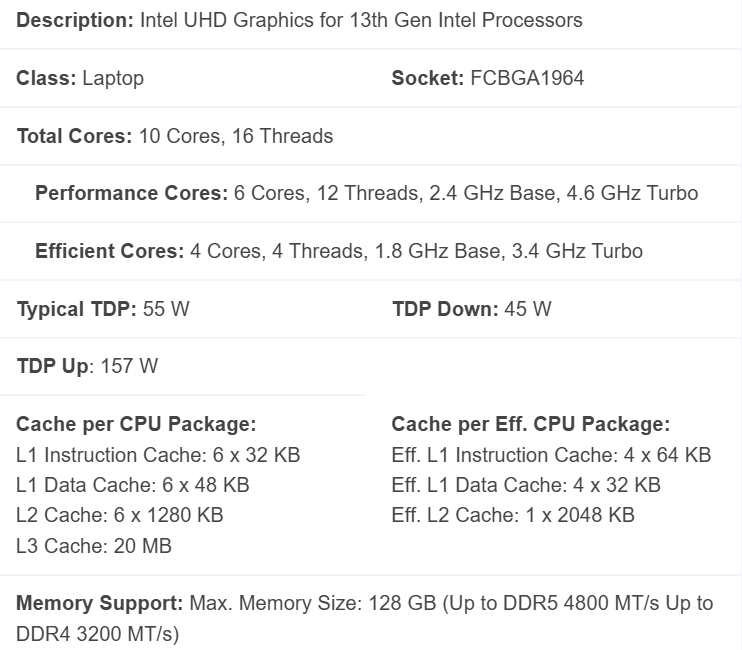
\includegraphics[width=\textwidth]{figures/processor.png}
        \end{column}
        
        % Coluna da Direita com as especificações detalhadas
        \begin{column}{0.6\textwidth}
            \textbf{Processador i5 13450HX (Laptop)}
            \vspace{0.2cm}
            \begin{itemize}
                \item \textbf{Arquitetura Híbrida:}
                    \begin{itemize}
                        \item 6 Núcleos de Performance (até 4.6 GHz) com 12 Threads
                        \item 4 Núcleos de Eficiência (até 3.4 GHz) com 4 Threads
                        \item \textbf{Total:} 10 Núcleos e 16 Threads
                    \end{itemize}
                \item \textbf{Memória Cache:}
                    \begin{itemize}
                        \item L3 Total: 20 MB
                        \item L2 Total: 9.5 MB
                    \end{itemize}
                \item \textbf{Memória Suportada:}
                    \begin{itemize}
                        \item DDR5 até 4800 MT/s
                        \item DDR4 até 3200 MT/s
                    \end{itemize}
            \end{itemize}
        \end{column}
    \end{columns}
\end{frame}


\begin{frame}{Desempenho do Algoritmo de Força Bruta (nanossegundos)}
    \centering
    { % Inicia um grupo para a mudança ser local
    \renewcommand{\arraystretch}{1.5} % <-- AQUI ESTÁ A MÁGICA!
    \begin{tabular}{|c|r|r|}
        \hline
        \textbf{N (Vértices)} & \textbf{Lista (ns)} & \textbf{Matriz (ns)} \\
        \hline
        8 & 68,833.60 & 2,428.82 \\
        \hline
        10 & 200,551.00 & 3,104.70 \\
        \hline
        12 & 655,799.00 & 3,146.28 \\
        \hline
        14 & 2,090,960.00 & 3,384.53 \\
        \hline
    \end{tabular}
    } % Termina o grupo
\end{frame}

\begin{frame}{Desempenho da Heurística de Grundy (milissegundos)}
    \centering
    { % Inicia um grupo para a mudança ser local
    \renewcommand{\arraystretch}{1.5} % <-- Aumenta a altura da linha
    \begin{tabular}{|c|r|r|}
        \hline
        \textbf{N (Vértices)} & \textbf{Lista (ms)} & \textbf{Matriz (ms)} \\
        \hline
        500 & 5.34 & 47.92 \\
        \hline
        1000 & 21.51 & 192.57 \\
        \hline
        2000 & 90.64 & 566.79 \\
        \hline
    \end{tabular}
    } % Termina o grupo
\end{frame}

\begin{frame}{Desempenho do Algoritmo de Força Bruta por Representação}
    \centering
    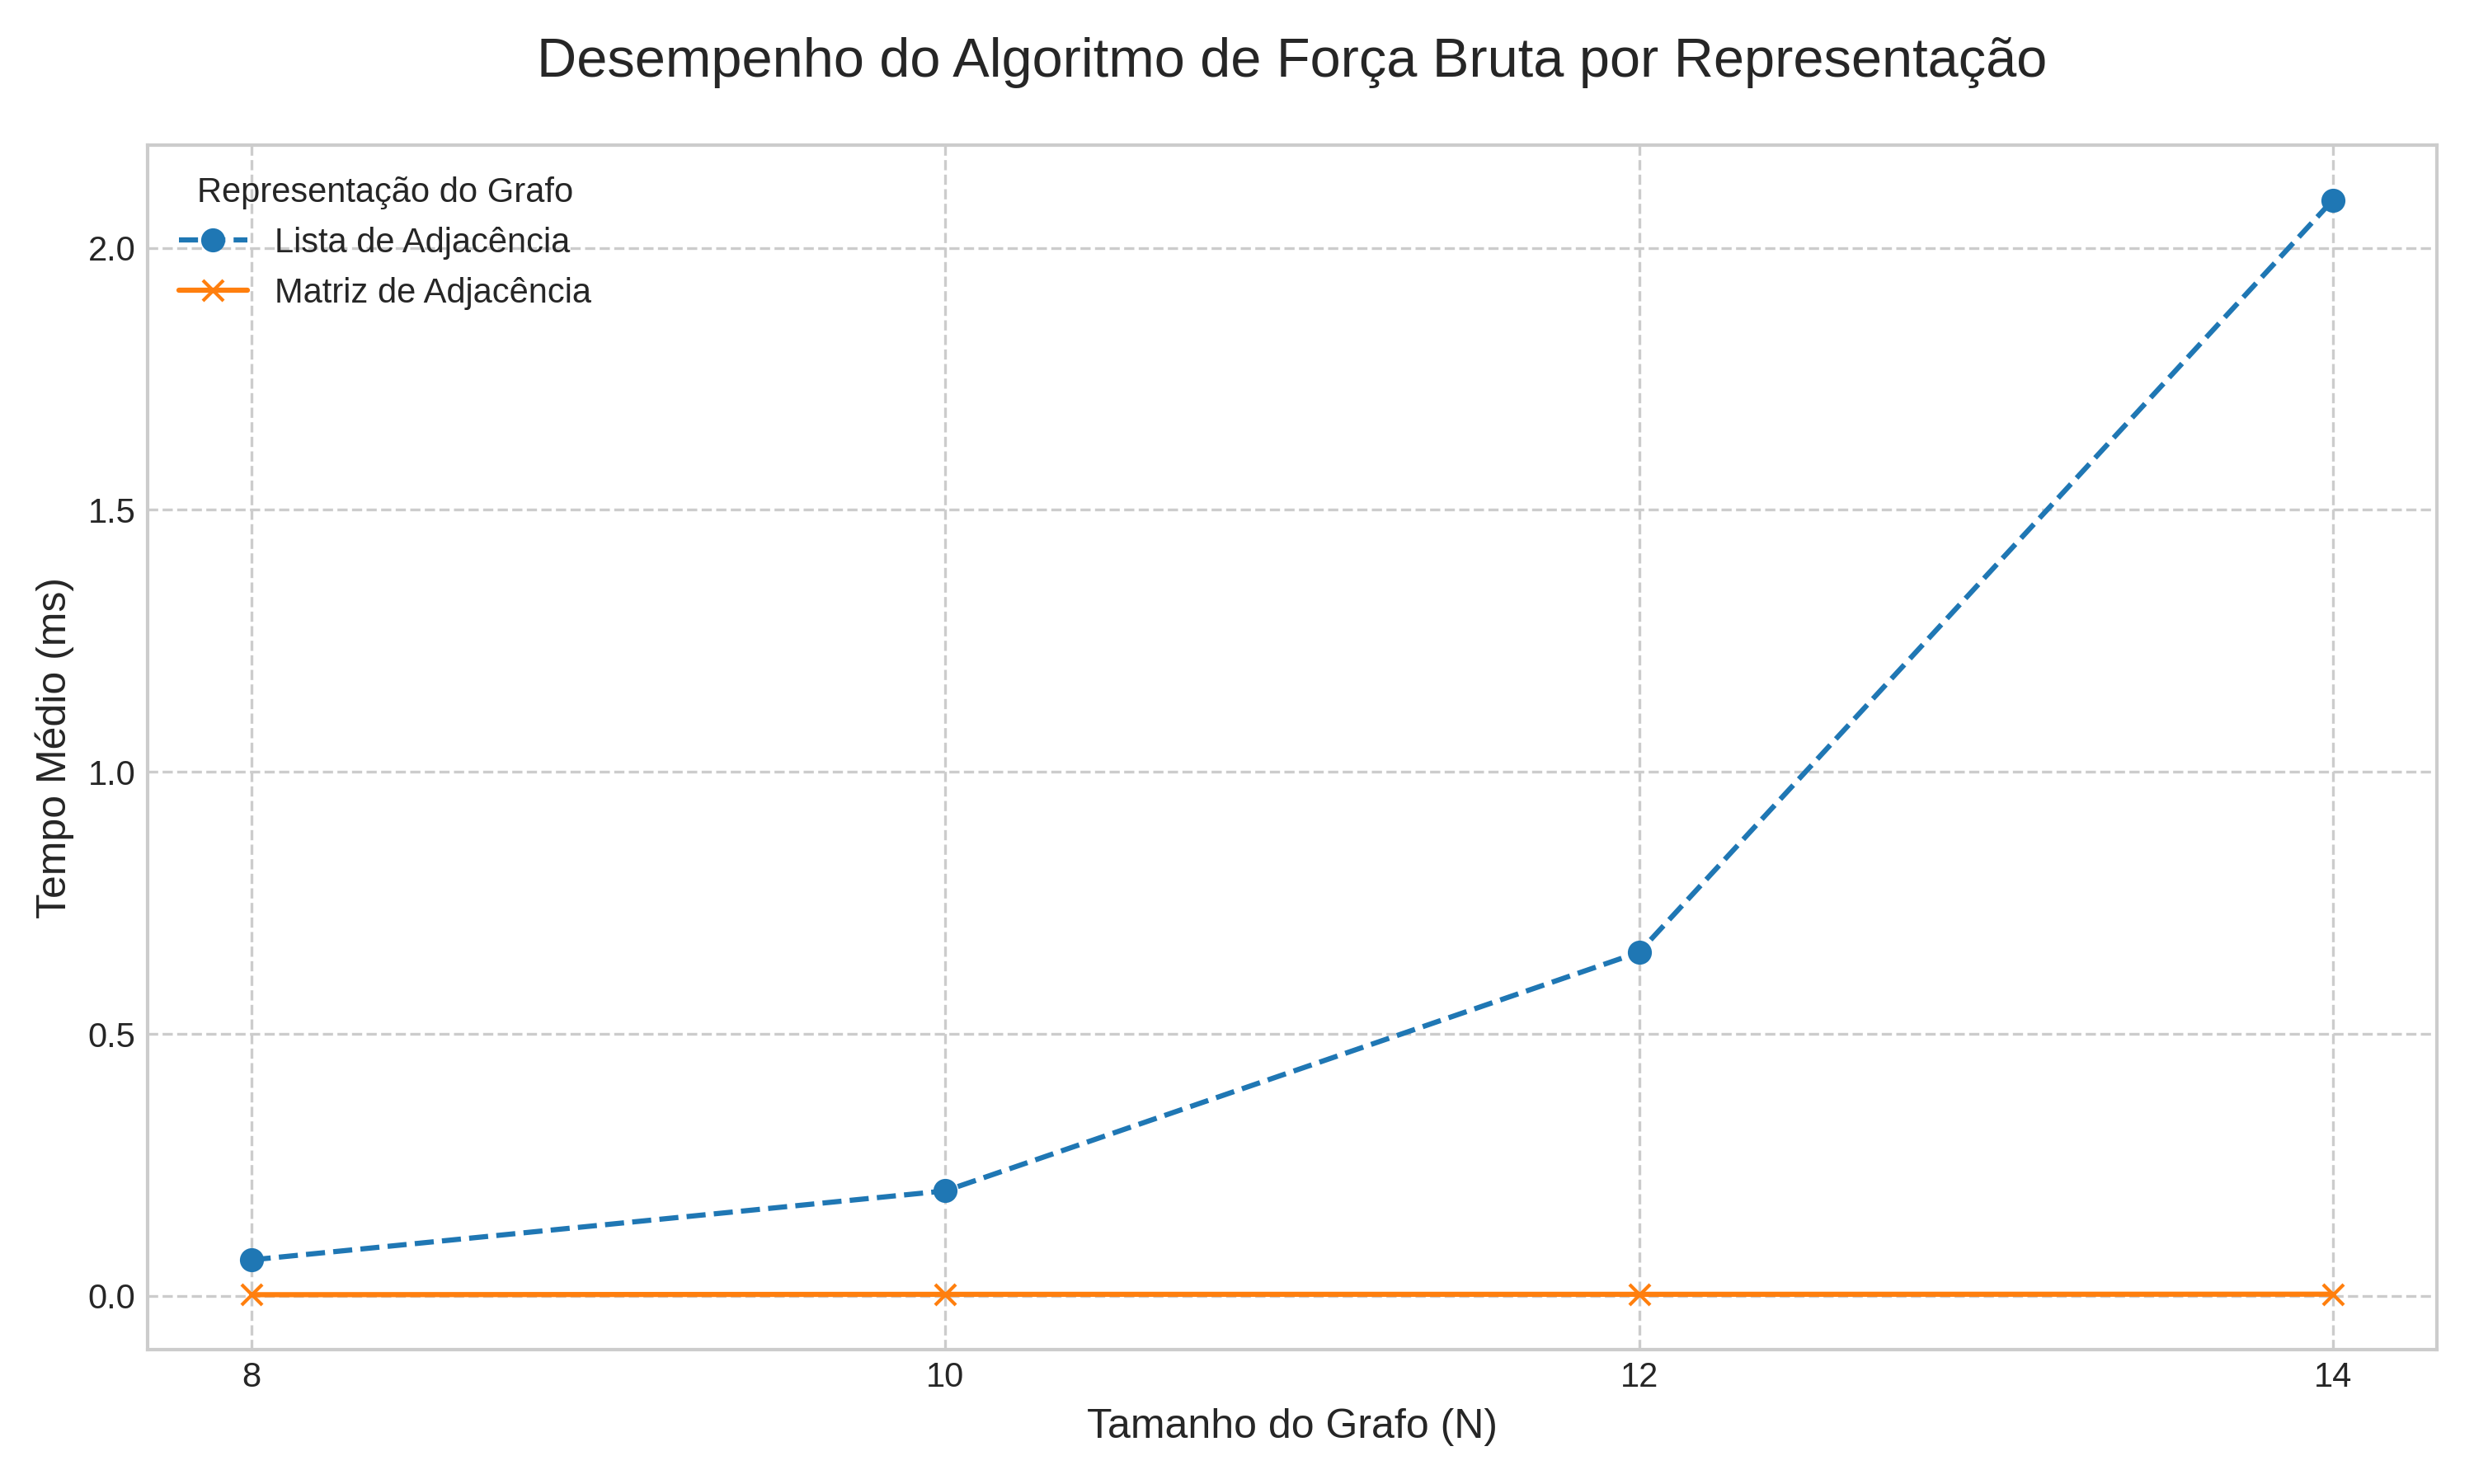
\includegraphics[width=0.9\textwidth]{figures/forca_bruta_comparativo.png}
\end{frame}

\begin{frame}{Desempenho do Algoritmo de Grundy por Representação}
    \centering
    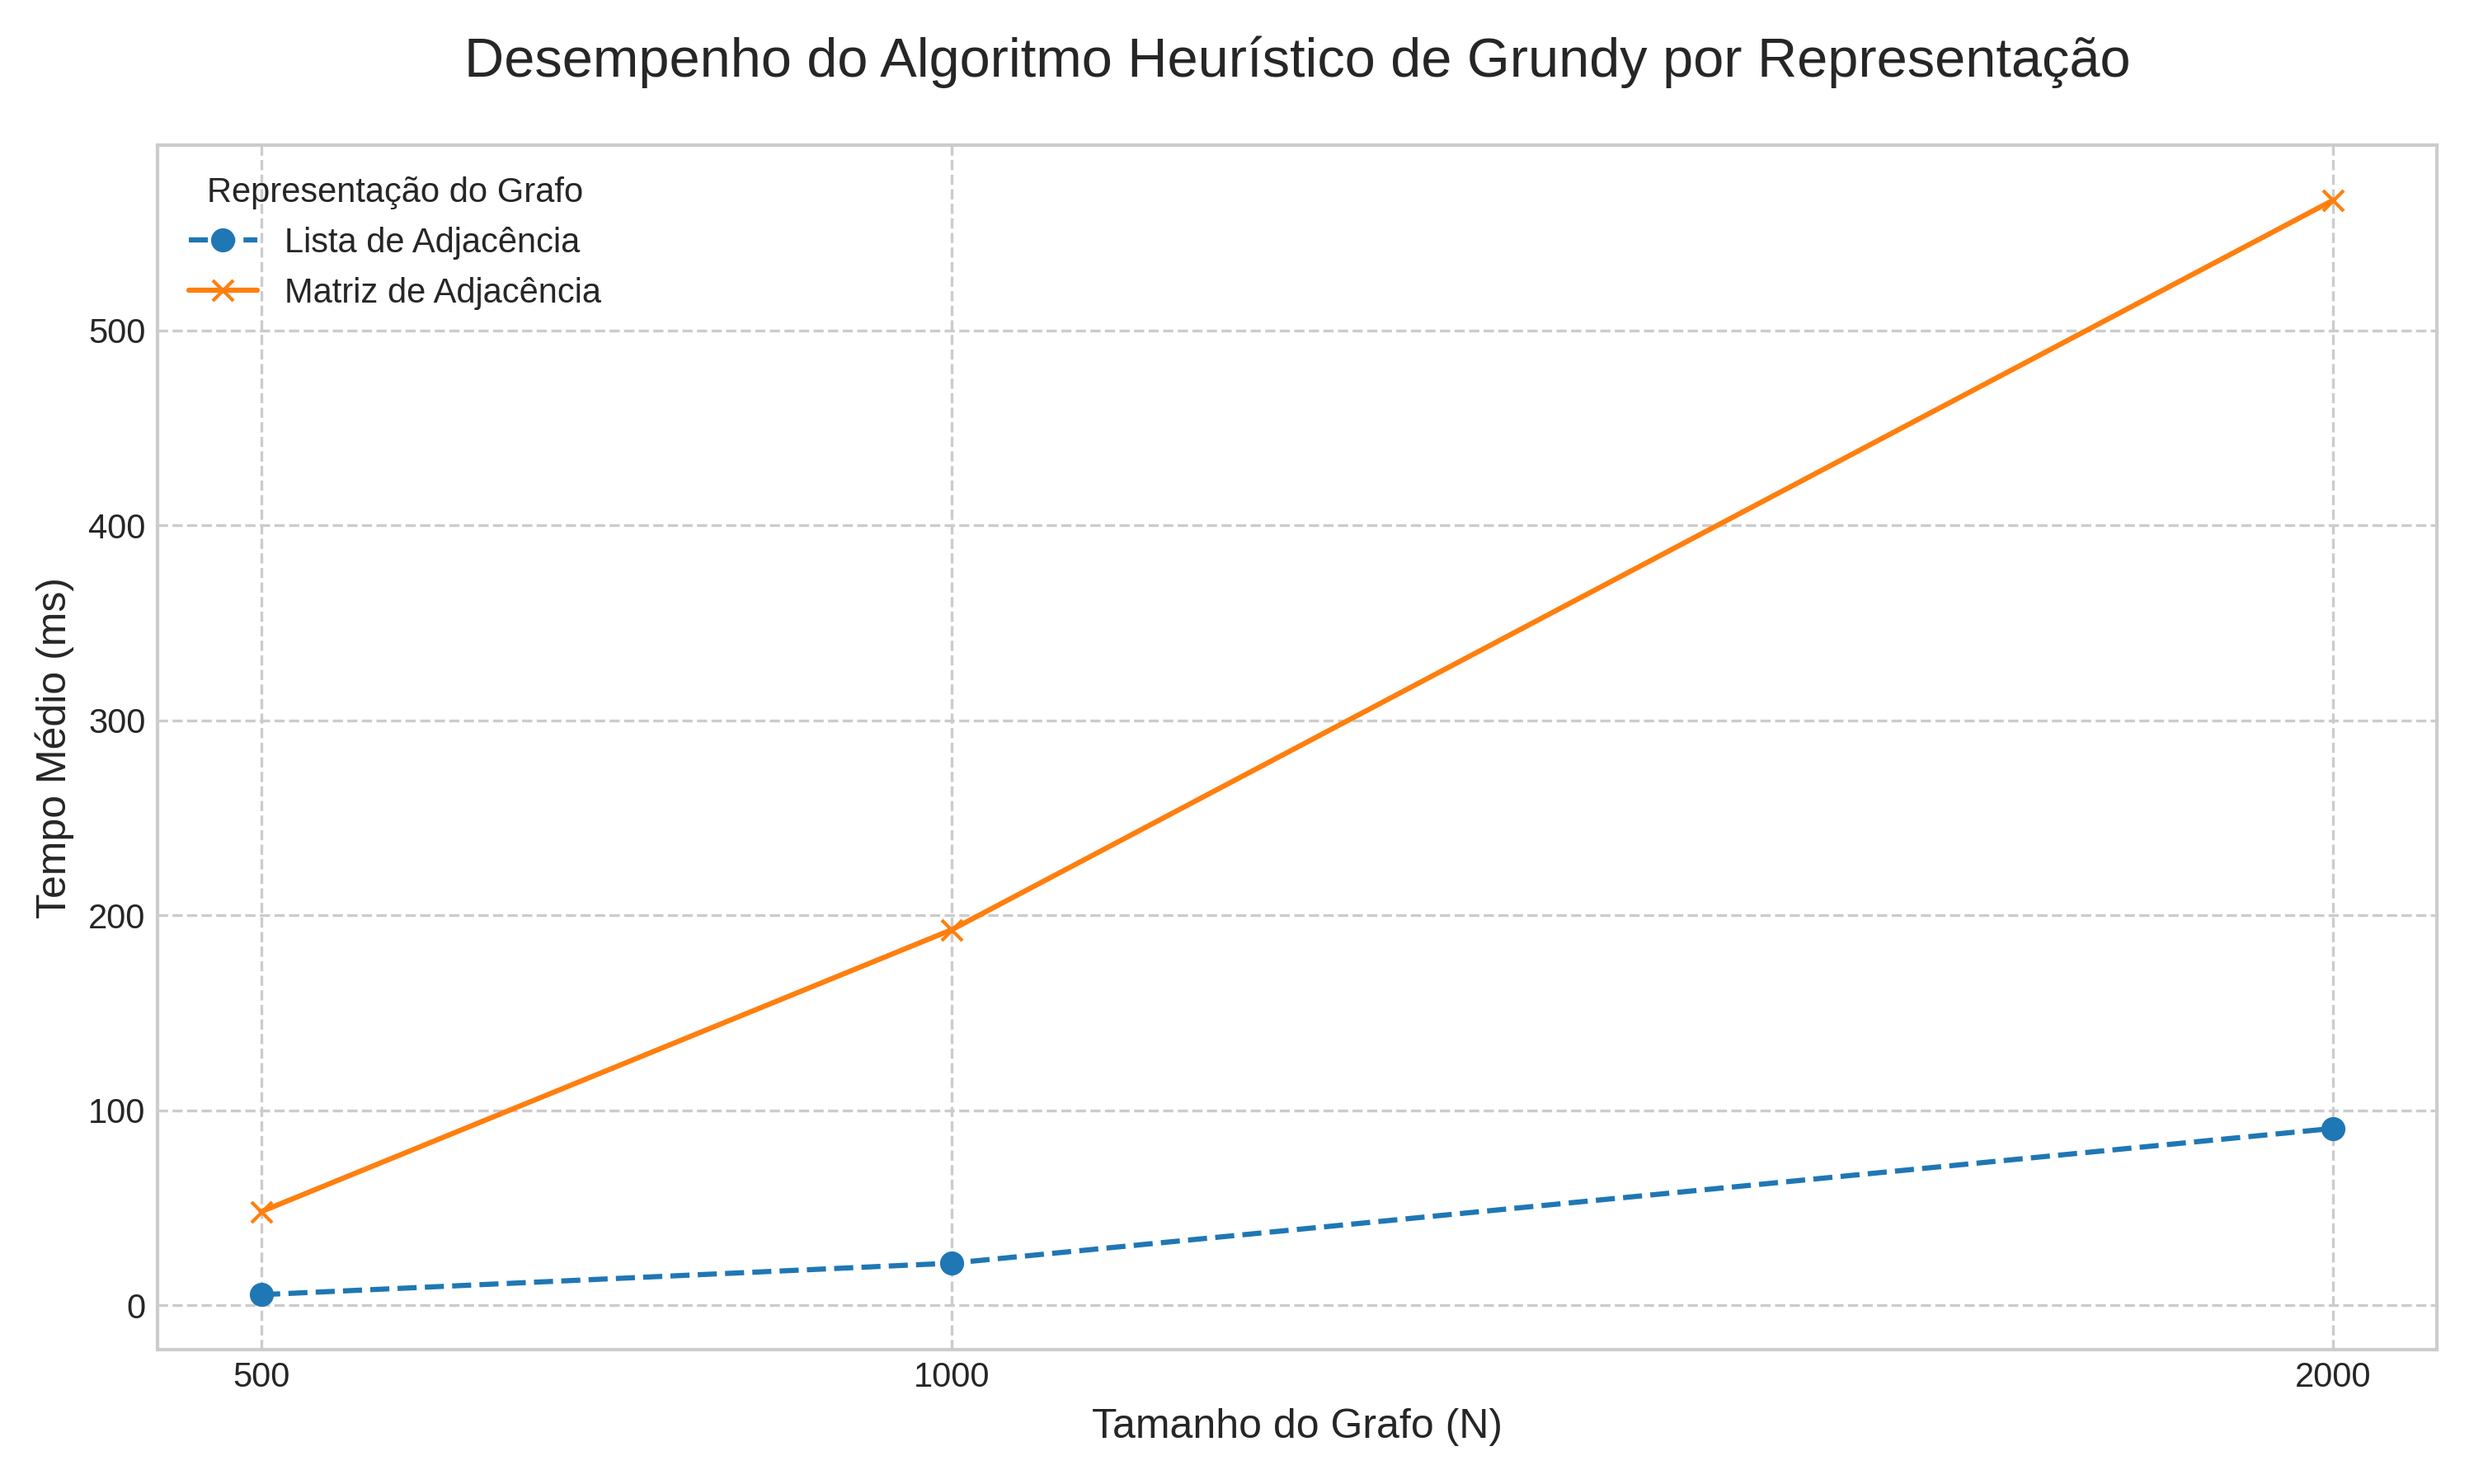
\includegraphics[width=0.9\textwidth]{figures/grundy_comparativo.png}
\end{frame}

\begin{frame}{Estimativas de Tempo para a Fase Grundy}
    \begin{itemize}
        \item Para 1.000 repetições (10 vezes mais que 100):
        \begin{itemize}
            \item $1,1 \text{ minutos} \times 10 = 11 \text{ minutos}$
        \end{itemize}
        
        \vspace{0.4cm}
        
        \item Para 10.000 repetições (100 vezes mais que 100):
        \begin{itemize}
            \item $1,1 \text{ minutos} \times 100 = 110 \text{ minutos}$
            \item Isso é aproximadamente 1 hora e 50 minutos.
        \end{itemize}
        
        \vspace{0.4cm}
        
        \item Para 1.000.000 de repetições (10.000 vezes mais que 100):
        \begin{itemize}
            \item $1,1 \text{ minutos} \times 10.000 = 11.000 \text{ minutos}$
            \item Convertendo para horas: $11.000 / 60 \approx 183,3 \text{ horas}$
            \item Convertendo para dias: $183,3 / 24 \approx 7,6 \text{ dias}$
        \end{itemize}
    \end{itemize}
\end{frame}